%!TEX root = ../../main.tex

\chapter{Grundlagen}
\label{chapter:3}

\section{Humanzentriertes Design}

Beim Entwickeln neuer Software setzen erfahrene Softwareentwickler häufig auf einen gut durchdachten Plan und Struktur. Dabei wird auf bestimmte Entwicklerprozesse gesetzt. Einer der bekanntesten Prozesse in der Softwareentwicklung ist hierbei der “Software Development Lifecycle” (kurz: SDLC). Der SDLC wird genutzt, um möglichst effiziente, kostengünstige Software mit hoher Qualität zu designen, entwickeln und produzieren.\cite{shylesh:2017} Es gibt eine Menge verschiedene Modelle des SDLC, jedoch haben alle Modelle im Grunde dieselbe Struktur: Planen - Designen - Implementieren - Testen. Besonders auf den Baustein “Design” soll in diesem Kapitel tiefer eingegangen werden.

Eine der weitverbreitetsten Designmodelle ist das “Human Centered Design” (kurz: HCD, dt.: menschenzentriertes Design).  Dabei handelt es sich um eine Designtechnik, bei der der Mensch im Vordergrund des Entwicklungsprozesses steht.\cite{hbsc:2020} Laut der Webseite der Harvard Business School liegen die Ziele des HCD darin, die Ziele, Wünsche und Vorlieben des Produktnutzers stetig im Auge zu behalten.\cite{hbsc:2020} Dort beschreibt ein Dekan der Harvard Business School vier grundlegende Phasen im HCD. Diese sind laut Dekan Srikant Datar folgende Phasen: Clarify - Ideate - Develop - Implement.\cite{hbsc:2020} Wiederum definiert Sim van der Ryn in seinem Paper “Human Centered Design” aus dem Jahr 2013 das Vorgehen des HCD ein wenig anders, jedoch ähnlich. Dieser schreibt, dass man sich zuerst mit dem potenziellen Nutzer beschäftigen sollte.\cite{vanderryn:2013} Anschließend wird das Problem definiert, eine Idee erarbeitet, ein Prototyp erstellt und abschließend getestet.\cite{vanderryn:2013}

\begin{figure}[h]
    \centering
    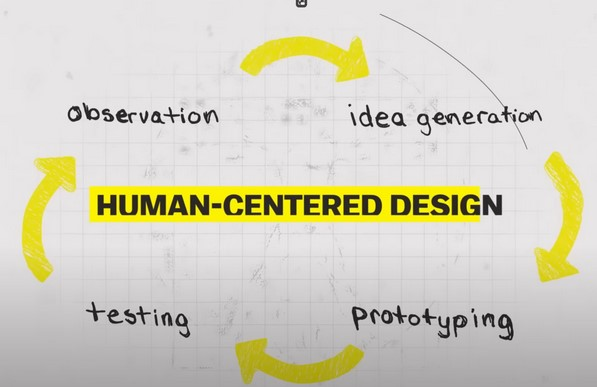
\includegraphics[width=1\textwidth]{images/03/HCD.jpg}
    \caption{Humand Centered Design Prozess}
\end{figure}

Zu den Vorteilen des HCD gehören unter anderem eine hohe Nutzerzufriedenheit, da die Meinung von Personen unmittelbaren Einfluss auf das Design des Produkts nehmen und so sicherstellen, dass alle Bedürfnisse und Erwartungen an das Produkt garantiert werden. Zudem kann dadurch auf die Wechselwirkung zwischen Menschen und Objekten besser verstanden werden, da man durch die Designfrage wichtige Erkenntnisse über das Verhalten bzw. Bedürfnisse der Menschen oder zumindest einer Personengruppe bekommt.

% ! Problem with Quote
% Zu den Vorteilen des HCD gehören unter anderem eine hohe Nutzerzufriedenheit, da die Meinung von Personen unmittelbaren Einfluss auf das Design des Produkts nehmen und so sicherstellen, dass alle Bedürfnisse und Erwartungen an das Produkt garantiert werden.\cite{hcd:2021} Zudem kann dadurch auf die Wechselwirkung zwischen Menschen und Objekten besser verstanden werden, da man durch die Designfrage wichtige Erkenntnisse über das Verhalten bzw. Bedürfnisse der Menschen oder zumindest einer Personengruppe bekommt.\cite{let:2022}

% ! Here too
Jedoch gibt es auch einige Nachteile bzw. Probleme des HCD. Ein Aspekt wäre die rapide Produktlebenszyklus. Durch die ständig wechselnden Bedürfnisse und Anforderungen an ein Produkt, stehen Designer und Designteams ständig unter großen Herausforderungen, um die Ansprüche treffen zu können. Häufig könnten aber auch eben diese menschlichen Anforderungen an ein Produkt zum Problem werden, da diese Anforderungen nicht umsetzbar und realisierbar sind.\cite{pod:2016}



\section{Nutzerzentriertes Design}
Achtet man nun beim Entwickeln neuer Software besonders auf den Nutzer und baut diese nach seinen Wünschen und Anregungen auf, so spricht man in diesem Fall von Nutzerzentriertem Design (kurz: UCD). Der wesentliche Unterschied zum Menschenzentrierten Design (HCD) ist jedoch, dass das Nutzerzentrierte Design soziale und kulturelle Aspekte nicht mit in das Design einfließen lässt.\cite{hcd2:2021} Diese Aspekt spielen beim Menschenzentrierten Design eine wesentliche Rolle. Dennoch wird UCD heutzutage auch mit HCD gleichgestellt.\cite{ucd1:2011}

Einer der zentralen Aspekte beim UCD sind so genannte Personas. Laut dem Buch "Persona Design in Participatory Agile Software Development" werden Personas häufig als Methode im UCD genutzt, um fiktionale Charaktere zu erschaffen, die verschiedene Nutzer bzw. gesamte Nutzergruppen zu repräsentieren.\cite{personaDesign:2020} Eine Persona wird dabei meistens in einer Erzählung beschrieben.\cite{ucd1:2011} Das Ziel liegt laut dem Artikel "Personas and user-centered design: How can personas benefit product design processes?" darin, die Persona wie eine reale Person darzustellen und die Bedürfnisse der Persona anschaulich innerhalb einer Gescichte darzustellen, um diese in die Entwicklung des Produktes einfließen zu lassen.\cite{ucd1:2011}
Grundsätzlich startet eine solche Erzählung mit einer Beschreibung der Person.\cite{ucd1:2011} Während der Beschreibung werden wichtige charakteristische Merkmale der Persona, wie z.B. Vorlieben und Abneigungen, Beruf etc. eingegangen.\cite{ucd1:2011}

\subsection{Erstellen einer Persona}
Die Erstellung einer Persona zählt zu den wesentlichen Punkten im UCD. In einem wissenschaften Paper der Universität Rostock wird der Bildungsprozess einer Persona beschrieben. Der komplette Entwicklungsprozesse einer Persona ist ebenfalls in der nachfolgenden Abbildung dargestellt:

\begin{figure}[h]
    \centering
    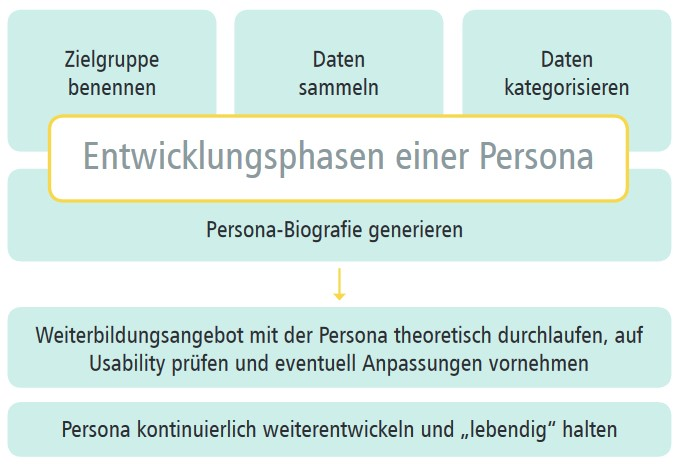
\includegraphics[width=1\textwidth]{images/03/entwicklungPersona.jpg}
    \caption{Entwicklungsprozess Persona \cite{personamethode}}
\end{figure}

Zu sehen ist, dass nahezu alle Schritte, welche vor der Erstellung von Personas passieren, mit Daten zutun haben. Besonders das Sammelen und Kategorisieren der Daten wird hier thematisiert.\cite{personamethode} Dazu schreibt der Wissenschaftler Frank Ploß in seiner Diplomarbeit "Usability Engineering in einem Open-Source-Projekt", welches ebenfalls von der Universität Rostock zitiert wird, dass es sich bei den eizenlenen Designstufen um iteratives Modell handelt.\cite{osp:masterthesis}
Das bedeutet im Grunde genommen nur, dass die einzelnen Schritte aufeinandner aufbauend sind. In dem Artikel wird zudem erwähnt, dass bereits im Vorfeld der Personaentwicklung Fragen über die Zielgruppe gestellt werden sollen, um die Erschaffung einer Persona zu vereinfachen.\cite{personamethode}
Diesen Schritt wird im Rahmen der Studienarbeit ausführlicher im Rahmen einer Umfrage durchgeführt.

Nachdem Sammeln und Kategorisieren der Daten wird die Persona definiert.\cite{personamethode} In diesem Schritt wird laut dem wissenschaftlichen Artikel der Universität Rostock eine Art Kurzbiografie für jede Persona erschaffen.\cite{personamethode} Als Beispiel für eine Persona in der Praxis verwendet die Universität Rostock deshalb Steckbriefe, um ihre Personas so kurz wie möglich, mit möglichst vielen Informationen darzustellen.\cite{personamethode}

Zum Abschluss sollten die Personas noch einen so genanntes Weiterbildungsangebot durchlaufen. Das bedeutet, dass man sich beispielsweise in die Sicht eines Kunden versetzt und als die gerade eben erstellte Persona den Einkaufsprozess durchläuft.\cite{personamethode} Dieser Schritt hilft dabei, die Persona noch stärker zu definieren und evtl. Schwächen/Stärken herauszufinden.
\section{Webtechnologien}

\subsection{Verwendung von React und anderen Webtechnologien in der App-Entwicklung}

\subsection{Technische Grundlagen der CO2-Runter-App}
